\documentclass[12pt, a4paper]{exam}
\usepackage{graphicx}
\usepackage[a4paper, total={6in, 8in}]{geometry}
\usepackage[normalem]{ulem}
\usepackage{amsmath}
\renewcommand\ULthickness{1.0pt}   
\setlength\ULdepth{1.3ex}

\begin{document}


	\noindent
	\begin{minipage}[l]{0.1\textwidth}
		\noindent
		
\includegraphics[width=2.8\textwidth]{ESCUDO.png}
	\end{minipage}
\hfill
\begin{minipage}[c]{0.8\textwidth}
	\begin{center}
		{\large  Departamento de Ingeniería civil y Agrícola\par
		\large	Facultad de Ingeniería	\par
	% \large \textbf{Taller propiedades de los fluidos}	\par
    \large \textbf{Taller de hisrost\'atica}	\par
} %%%%% NOMBRE DEL PROFESOR 
	\end{center}
\end{minipage}
\par
\vspace{0.2in}
\noindent
    \uline{Mecánica de fluidos [2015966]	\hfill 2022-II	}
\par 
\vspace{0.15in}
\noindent
\centering


\begin{questions}

    \question Las unidades de energía en el sistema inglés de unidades están dadas por (lbf pie). Convierta una unidad de energía en este sistema al sistema internacional de unidades.

	\question Si el peso específico de un gas es 12.4 $N/m^3$, ¿Cuál es su volumen específico en $m^3/kg$?
		
   \question

    Un objeto pesa 300 N en la superficie de la tierra Determine la [masa del objeto en kilogramos y su peso en newtons cuando este objeto es llevado a otro planeta con una aceleración de la gravedad igual a 4.0 ft/s$^2$. Justifique su respuesta.
  
    \question ¿Cuál de las siguientes unidades de medida pertenece al Sistema Internacional de Unidades (SI)? Justifique su respuesta. 
    
    \begin{parts}
    \part Milla 
    \part Milímetro
    \part Pie 
    \end{parts}
    
    %%% PUNTO 14
    \question ¿Cuál de las siguientes unidades de medida no pertenece al sistema de unidades inglés (o imperial)? Justifique su respuesta. 
    
    \begin{parts}
    \part Libra
    \part Litro
    \part Yarda
    \end{parts}

    \question Un contenedor cónico invertido, cuyo diámetro es 26 pulgadas y altura 44 pulgadas esta lleno con un líquido a $ 20^{o}$ C. El peso del liquido son 5030 onzas. ¿Cual es la densidad del fluido en kg/m3?

    \question La viscosidad absoluta (o dinámica) del mercurio es de 1.7 cP y su gravedad específica es de 13.6 a temperatura y presión atmosférica estándar.Encuentre la viscosidad cinemática en el sistema internacional y en sistema ingles.
    
    \question Si un tanque con aceite pesa 1.5 kN , calcular el peso específico la densidad y la gravedad específica del aceite. El barril contiene 159 litros y pesa 110 N cuando esta vacío. 
    
    \question Determine el peso y la gravedad específica de un galón de líquido, si este tiene una masa de 0.258 slug. Exprese todas las variables en el sistema inglés.
    
    \question Para flujo permanente en una tubería circular a velocidad baja, la velocidad u varía como:
    
    \begin{equation}
    u=B\frac{\Delta_{p}}{\mu }(r_{0}^{2}-r^{2})   
    \end{equation}
    
    donde r es el radio de la tubería, $\mu$ es la viscosidad del fluido y $\delta_p$ es el cambio de presión a lo largo de la tubería. ¿Cuales son las dimensiones de la constante B?

    \question En 1908, Heinrich Blasius estudiante de Prandtl, propuso la siguiente fórmula para los esfuerzos cortantes ($\tau_w$) de un fluido viscoso:
    
    \begin{equation}
    \tau_w=0.332\rho ^{1/2}\mu ^{1/2}V^{3/2}x^{-1/2}   
    \end{equation}
    
    en donde V es la velocidad, $\rho$ es la densidad, $\mu$ es la viscosidad y x es una distancia recorrida. Determine las dimensiones de la constante 0.332.
    
	\question Un orificio se define como una perforación por debajo de una superficie libre de un líquido, ya sea ubicado en la pared o en el fondo de un depósito cualquiera (tanque, canal, depósito), a través, del cual se evacua el líquido almacenado mediante la siguiente ecuación:
	\begin{equation}
    Q=C_{d}A\sqrt{2gh}
    \end{equation}
    
	Donde, Q es el caudal, $C_d$ es el coeficiente de descarga de un orificio (adimensional), A el área, g la aceleración de la gravedad y h la carga hidráulica.
	
    \begin{figure}[h]
    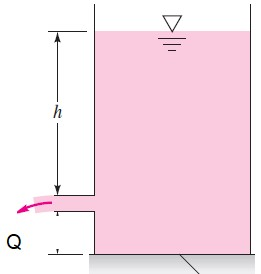
\includegraphics[width=4cm]{CAUDAL P1.jpg}
    \centering
    \end{figure}

	Demuestre que la Ecuación 1 es:
	
	\begin{parts}
		\part Dimensionalmente homogénea  \textbf{\droppoints}
		\part Consistente en el Sistema Ingles.\textbf{\droppoints}		
	\end{parts}

	\question La fórmula hidráulica de Hazen-Williams para el caudal volumétrico Q a través de una tubería de diámetro D y longitud L está dada por:
	
	\begin{equation}
    Q \simeq 61.9 D^{2.63} \left( \frac{\Delta_{P}}{L} \right)^{0.54}
    \end{equation}	
		
	donde $\Delta_p$  es la caída de presión requerida para impulsar el flujo.
	\vspace{0.2in}
	\begin{parts}
		\part  ¿Cuáles son las dimensiones de la constante 61.9? 
		
	\end{parts}
	
    \question Un líquido vertido en un recipiente cilíndrico con marcas de graduación (por ejemplo, la licuadora muestra graduación en tazas) registra que el volumen es de 500 ml y pesa 8N. Determinar su peso específico, densidad y gravedad específica.

    \question Un líquido tiene un peso específico de 59 lb/ft y una viscosidad dinámica de 2.75 lb.s/ft$^2$. Determinar la viscosidad cinemática en m$^2$/s. 
    
	\question Un eje lubricado rota dentro de una camisa concéntrica a 2000 $rpm$. La luz $\delta$ es pequeña respecto al radio $R$. 
	\vspace{0.2in}
	\begin{parts}
		\part ¿Cuáles son los requerimientos de potencia para rotar el eje? R = 2 pulgadas, L= 6 pulgadas, $\delta$ = 0.1 mm y $\mu$ = 0.3 $N s/m^{2}$. 
		\textbf{\droppoints}

    \begin{figure}[h]
    \includegraphics[width=9cm]{eje.jpg}
    \centering
    \end{figure}		
		
	\end{parts}


 %%%% PUNTO 6
 
 %%%%%  A block of weight W slides down an inclined plane while lubricated by a thin film of oil, as in Fig P1.45. The film contact area is A and its thickness is h. Assuming a linear velocity distribution in the film, derive an expression for the “terminal” (zero-acceleration) velocity V of the block. Find the terminal velocity of the block if the block mass is 6 kg, A=35 cm 2 , θ=15°, and the film is 1-mm-thick SAE 30 oil at 20°C
 
	\question Un bloque de peso W se desliza por un plano inclinado mientras está lubricado por una película delgada de aceite, como en la Figura a continuación. El área de contacto de la película es A y su espesor es h. Suponiendo una distribución de velocidad lineal en la película, obtenga una expresión para la velocidad "terminal" (aceleración cero) V del bloque. Encontrar la velocidad terminal del bloque si la masa del bloque es de 6 kg, A=35 cm 2 , $\theta$=15°, y la película es de 1 mm de espesor SAE 30 a 20°C
	

    \begin{figure}[h]
    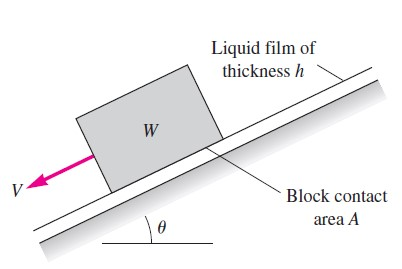
\includegraphics[width=9cm]{BLOQUE.jpg}
    \centering
    \end{figure}		

 %%%% PUNTO 7
 
 %%%%% A thin plate is separated from two fixed plates by very viscous liquids mu1 and mu2, respectively, as in Fig. P1.48. The plate spacing h1 and h2 are unequal, as shown. The contact area is A between the center plate and each fluid. (a) Assuming a linear velocity distribution in each fluid, derive the force F required to pull the plate at velocity V. (b) Is there a necessary relation between the two viscosities, mu1 and mu2? 
 
	\question Una placa delgada está separada de dos placas fijas por líquidos muy viscosos $\mu$1 y $\mu$2, respectivamente, como en la figura P1.48. El espaciamiento de las placas h1 y h2 son desiguales, como se muestra. El área de contacto es A entre la placa central y cada fluido.
    \begin{figure}[h]
    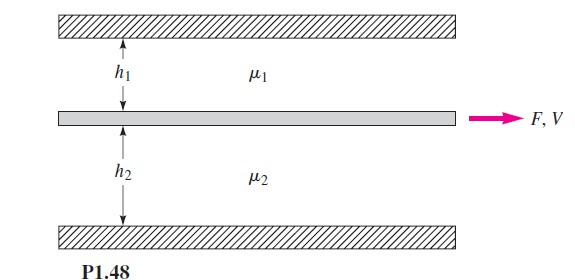
\includegraphics[width=9cm]{1.48 .jpg}
    \centering
    \end{figure}		

	\begin{parts}
		\part Suponiendo una distribución de velocidad lineal en cada fluido, obtenga la fuerza F (fuerza de corte) requerida para tirar de la placa a la velocidad V.
		\part  ¿Existe una relación necesaria entre las dos viscosidades, $\mu$1 y $\mu$2?.
	\end{parts}


 %%%% PUNTO 8
 
 %%%%% A solid cone of angle 2θ, base r 0 , and density ρc is rotating with initial angular velocity ω0 inside a conical seat, as shown in Fig. P1.53. The clearance h is filled with oil of viscosity μ. Neglecting air drag, derive an analytical expression for the cone’s angular velocity ω(t) if there is no applied torque.
 
 
	\question Un cono sólido de ángulo 2$\theta$, base $r_0$ y densidad $\rho_c$ gira con una velocidad angular inicial $\omega_0$ dentro de un asiento cónico, como se muestra en la figura P1.53. El espacio h está lleno de aceite de viscosidad $\mu$. Despreciando la resistencia del aire, obtenga una expresión analítica para la velocidad angular del cono $\omega(t)$ si no se aplica un par de torsión.
    \begin{figure}[h]
    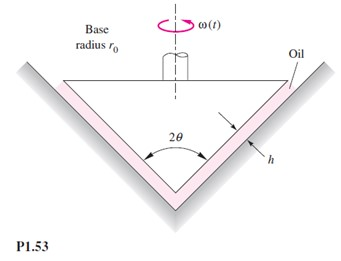
\includegraphics[width=9cm]{1.53.jpg}
    \centering

    \end{figure}		
\newpage

 %%%% PUNTO 9
 
 %%%%% A disk spins within an oil-filled enclosure, having 2.4 mm clearance from flat surfaces each side of the disk. The disk surface extends from radius 12 to 86 mm. What torque is required to drive the disk at 660 rpm if the oil's absolute viscosity is 0.12 N s/m^2?
 
	\question Un disco gira dentro de un recinto lleno de aceite, con una separación de 2,4 $mm$ de las superficies planas a cada lado del disco. La superficie del disco se extiende desde un radio de 12 a 86 $mm$. ¿Qué par de torsión se requiere para impulsar el disco a 660 $rpm$ si la viscosidad absoluta del aceite es de 0,12 $N s/m^2$?
    %%% PUNTO 4 
    
	\question  Derive la expresión para el cambio de altura h en un tubo circular de un líquido con tensión superficial Y y el ángulo de contacto $\theta$.
		
    \begin{figure}[h]
    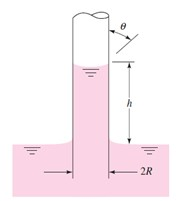
\includegraphics[width=5cm]{TUBO.jpg}
    \centering
    \end{figure}

   %%% PUNTO 26
    \question A presión atmosférica $ P_{atm} $ = 14.7 psi, un tanque contiene 120 $pie^{3}$ de agua que pesa 7488 lb. El módulo de elasticidad volumétrico del agua es de 300000 psi. Determine:
    \begin{parts}
        \part Su densidad.
        \part Si la presión se eleva a 1470 psi, ¿cual es el valor de la densidad?
        \part ¿que presión se requiere para reducir su volumen en 0.5\%?
    \end{parts}
    
   %%% PUNTO 27
 

   %%% PUNTO 28
    \question Si el volumen de un líquido es reducido en 0.035\%? mediante la aplicación de una presión de 690 $kPa$ o 100 $psi$, ¿cual es el módulo de elasticidad?
 %%%% PUNTO 10
 %%%%% Water at 170 F in a beaker is placed within an airthight container. Air is gradually pumped out of the container. What reduction below standart atmospheric pressure of 14.7 psia must be achieved before the water boils?
 
	\question Se coloca agua a 170 F en un vaso de precipitados dentro de un recipiente hermético. El aire se bombea gradualmente fuera del contenedor. ¿Qué reducción por debajo de la presión atmosférica estándar de 14,7 psia debe lograrse antes de que hierva el agua?

 \question 	Un fluido newtoniano tiene una gravedad específica de 0.92 y una viscosidad cinemática de 4 x 10-4 m2/s que fluye con una placa fija. El perfil de velocidades cerca de la superficie se muestra en la figura. Determine la magnitud y dirección de un esfuerzo de corte que se desarrolla en la placa fija. Exprese su respuesta en términos de U [m/s] y de $\delta$ [m].
 \begin{figure}[h]
    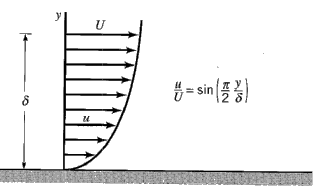
\includegraphics[width=8cm]{perfilVel.png}
    \centering
    \end{figure}

 \question 	El tanque cerrado en la figura siguiente está a una temperatura de 20°C. Si la presión en A es 95 kPa (abs), determine la presión (abs) en B. ¿Qué porcentaje de error usted tendría si desprecia el peso específico del aire?
 \begin{figure}[h]
    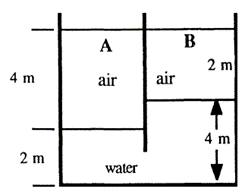
\includegraphics[width=5cm]{aguaAire.png}
    \centering
    \end{figure}
    
\question Se tiene una burbuja de 2.5 cm de radio de agua jabonosa con una tensión superficial de 32 mN/m. Se sopla hasta formar un radio de 4.5 cm. Calcule el trabajo efectuado para estirar la superficie de la burbuja y exprese su respuesta en Julios.

% Ejercicios de gases, by LAM (26/08/22)    
\question Un gas de peso molecular 44 ocupa un volumen de 4 $pie^3$ cuando la presi\'on y la temperatura absoluta son de 2000 $lb/pie^2$ y 600 $^o$R respectivamente. Calcule su volumen espec\'ifico y su peso espec\'ifico.

\question Un metro cubico de nitr\'ogeno a 40 $^o$ y 340 kPa es comprimido isoentropicamente a 0.2 $m^3$.¿Cual es la presi\'on y la temperatura cuando el nitr\'ogeno es reducido a este volumen? ¿Cual es el m\'odulo de elasticidad antes y despu\'es de la compresi\'on? $k =$1.4 y la constante del gas $R =$296.5 $\frac{N.m}{kg. ^oK}$.

\question Se tiene aire ($k =$ 1.4) a presion de 3 $kg/cm^2$ cuando su volumen es de 0.4 $m^3$. ¿Cual ser\'a su presi\'on final y su m\'odulo de elasticidad volum\'etrica cuando se comprime hasta 0.1 $m^3$?. Encuentre estos valores cuando: a) se considera un proceso isot\'ermico bajo una temperatura de 50 $^o$C; b) se considera un proceso isoentr\'opico. Luego determine la temperatura final del aire.



\end{questions}


\end{document}


